\subsection{Constraints from perturbativity and unitarity}

%\del{To perform well established perturbative calculations we require that all the quartic couplings in the scalar potential (\ref{potential}) obey the condition 
%\begin{equation}
%\label{eq:pert}
%|\lambda_i|\leq 8\pi. 
%\end{equation}
%
%
%We start our exploration of the I2HDM parameter with the following wide scan for the 
%five model parameters indicated above including $\lambda_{345}$ and $\lambda_2$
%range for which is limited by perturbativity requirement:
%\begin{table}[ht]
%\begin{center}
%\begin{tabular}{|c|c|c|}
%\hline
%Parameter      & min value &  max value \\ \hline 
%Mh$_1$ [GeV]   &    10	&     1000  \\ \hline
%Mh$_2$ [GeV]   &    10	&     1000  \\ \hline
%Mhc [GeV]      &    10	&    1000  \\ \hline
%$\lambda_{345}$&  $-8\pi$  &    $8\pi$  \\ \hline
%$\lambda_2$    &   $-8\pi$ &     $8\pi$   \\ \hline
%\end{tabular} 
%\end{center}
%\caption{Range for the wide scan of the parameter space. \giac{}{COMMENT: I would present this table when showing the results of the scan. Is this the range used?} \label{tab:wide-scan}}
%\end{table}
%}

The first requirement we impose on the quartic couplings in (\ref{potential}) is that their values are such that perturbative calculations can be trusted in the model.  The most effective way is to impose perturbative unitarity on all the scattering processes involving the scalars.
Following~\cite{Arhrib:2012ia}, we impose this condition on the full scattering matrix, which leads to the following bounds on combinations of couplings $e_i$:
%
\begin{equation}
\label{eq:unit}
|e_i|\leq 8\pi\,,
\end{equation}
where
$e_{1,2}= \lambda_3 \pm \lambda_4, \ \ e_{3,4}=\lambda_3 \pm \lambda_5, \ \ \
e_{5,6}= \lambda_3 + 2\lambda_4 \pm 3\lambda_5, \ \ \  e_{7,8} = -\lambda_1-\lambda_2 \pm \sqrt{(\lambda_1-\lambda_2)^2+\lambda_4^2}$, $e_{9,10} = -3\lambda_1 - 3\lambda_2 \pm \sqrt{9(\lambda_1 -\lambda_2)^2 + (2\lambda_3+\lambda_4)^2}, \ \ \ 
 e_{11,12} = -\lambda_1 - \lambda_2 \pm \sqrt{(\lambda_1 - \lambda_2)^2 + \lambda_5^2}
$.
The parameter $\lambda_1$ is fixed by SM-Higgs mass and the vacuum expectation value.
One can verify that the constraints given by Eq.~(\ref{eq:unit}) imply that all quartic couplings in (\ref{potential}) are bound to be smaller than $8\pi$, thus within the perturbative regime.
The perturbativity constraints can also be used to find upper bounds on the two input couplings we defined in the previous section, i.e. $\lambda_2$ and $\lambda_{345}$. From $e_{10}$ one finds:
\begin{equation}
\lambda_2<\lambda_2^{max} < 4\pi/3,
\end{equation}
where $\lambda_2^{max}$ is a function of  model parameters,
while from $e_5 = 3 \lambda_{345} - (2 \lambda_3 + \lambda_4)$, combined with $e_{10}$ in the limit $\lambda_2 = 0$, we obtain an upper bound for $\lambda_{345}$:
\begin{equation}
- 1.47 \simeq -2\sqrt{\lambda_1 (4\pi/3)} < -2\sqrt{\lambda_1\lambda_2^{max}}<\lambda_{345}\lessapprox {2\over 3} \times 8\pi - \lambda_1,
\label{eq:l345min}
\end{equation}
where we expanded at leading order in the small coupling $\lambda_1$, and the lower bound comes from the stability of the potential.
This limit, derived from the constraints on $e_5$ and $e_{10}$ is not actually the most stringent one:
in the limit of $\lambda_2 \to 0$ we have found  that the biggest value for $\lambda_{345}$
is realised in the  $|\lambda_{4,5}| \to 0$ limit when $\lambda_3 \simeq  4\pi$ 
and respectively  $\lambda_{345} \simeq 4\pi$.
After expansion in  the small coupling $\lambda_1$, the upper limit on  $\lambda_{345}$ in the small $\lambda_2 $ limit 
reads as 
\begin{equation}
\lambda_{345}\lessapprox 4\pi-{3\over 2}\lambda_1
\label{eq:l345max}
\end{equation}
while for finite  $\lambda_2 $ the limit can be found numerically.

One should also stress  that the vacuum stability condition given by  Eq.(\ref{eq:scalar-pot2})
sets an important constraint on the  maximum value of $\lambda_{345}$
in the small  $M_{h_1}$ region (which is the region of our special interest
because of the collider phenomenology constraints as we discuss below).
This can be seen from Eq.(\ref{eq:scalar-pot2}) which can be written 
as:
\begin{equation}
\lambda_{345}< 2\left(\frac{M_{h_1}^2}{v^2}+\sqrt{\lambda_1\lambda_2^{max}}\right)
\label{eq:l345-vacuum-stab}
\end{equation}
 
%
In Fig.\ref{fig:par-space1},
we present viable parameter space in the ($\lambda_{345},\lambda_2$) plane
after 
constraints from Eq.~(\ref{eq:unit}) as well constraints from 
scalar potential given by Eqs.~(\ref{eq:scalar-pot1}),~(\ref{eq:scalar-pot2}),~(\ref{eq:l345-vacuum-stab}).
%
\begin{figure}[htb]
\centering
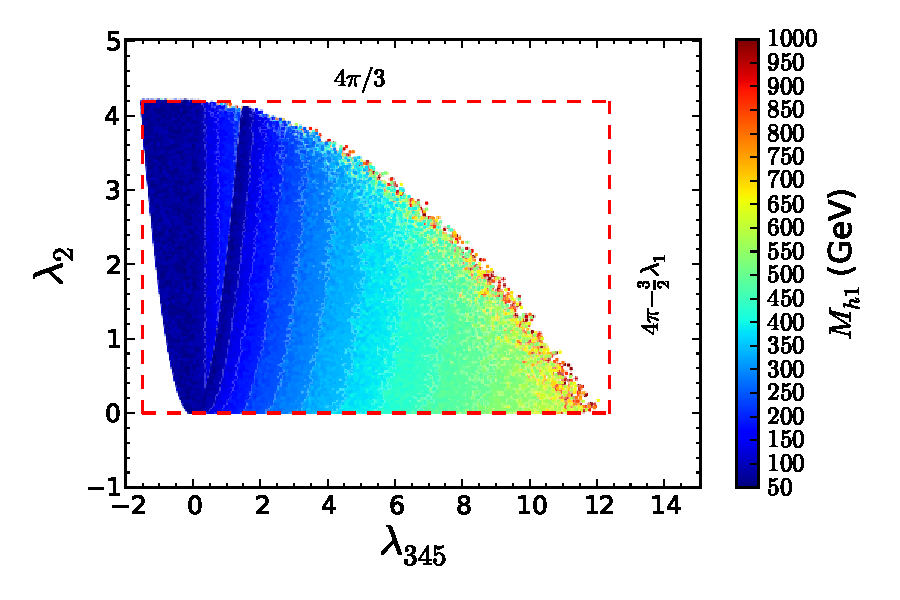
\includegraphics[width=0.7\textwidth]{Figures/l345_ld_cut12_c.pdf}
\caption{The part of the ($\lambda_{345},\lambda_2$) parameter space 
allowed by the unitarity, perturbativity and scalar potential constraints.\label{fig:par-space1}}
\end{figure}
To produce this plot we have performed the wide random scan to cover  the full five-dimensional  parameter space of the model,  with the following chosen 
range for the  model parameters:
\begin{eqnarray}
10\mbox{ GeV} < &M_{h1,h2,h^+}& < 1000 \mbox{ GeV} \nonumber\\
0< &\lambda_2& < {4\pi\over 3} \nonumber\\
-1.47 < &\lambda_{345}& < 4\pi 
\label{eq:scan-limits}
\end{eqnarray}
The colour map in Fig.~\ref{fig:par-space1} presents the values for the third essential parameter,
the DM candidate mass $M_{h_1}$,
with points  of smaller values of $M_{h_1}$ on the top of points with larger   $M_{h_1}$ values.
From this figure one can observe a non-trivial shape of the allowed parameter space in the 
($\lambda_{345},\lambda_2$) plane defined by the constraints mentioned above. In particular,
for small  $M_{h_1}$ values, the upper limit on $\lambda_{345}$
comes from Eq.(\ref{eq:l345-vacuum-stab}) which restricts $H h_1 h_1$ coupling 
$\lambda_{345}$ to be not very large.
The value of $\lambda_2^{max}$ entering there can be found in general only numerically.  







